\documentclass[../main.tex]{subfiles}
\graphicspath{{\subfix{images/}}}

\begin{document}
	\section{Sorting networks preliminaries}
	A comparator network with n inputs is a sequence of comparators, each comparator is formed by a tuple of channels $C=(i_1,j_1);...;(i_k,j_k)$ where $(1 \leq i_l < j_l \leq n)$. We name size k to the number of comparators the network has. An input $\bar{x}=x_1...x_n \epsilon \{0, 1\}^n$ outputs the network as follows: $\bar{x_0}=\bar{x}$ for $0<l\leq k$, $\bar{x^l}$ is a permutation of $\bar x^{l-1}$ exchanging $\bar x^{l-1}_{i_l}$ and $\bar x^{l-1}_{j_l}$ if $\bar x^{l-1}_{i_l} > \bar x^{l-1}_{j_l}$
	A comparator network is a sorting network if for any n inputs the outputs are the ascending ordered sequence. The reason we take only binary sequences is because of the zero-one principle\cite{knuth1997art} which states that a comparator network orders all sequences in \{0,1\} if and only if it sorts all sequences in any ordered set such as the integers set. This also allows to test if a comparator network is a sorting network without testing n! combination of sequences. If a comparator network tests all the binary sequences in 1-n it is enough to state that it is indeed a sorting network.
	
	\begin{figure}[H]
		\centering
		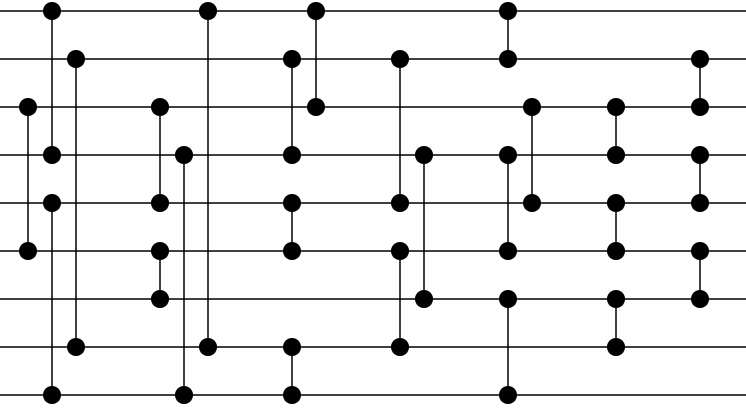
\includegraphics[scale=0.8]{images/Size8SortingNetwork}
		\caption{Size 8 sorting network}
		\label{fig:images/Size8SortingNetwork}
	\end{figure}

	As stated before the creation of sorting networks with optimal size is the problem of finding networks with the smallest possible set of comparators. Until this date optimal size sorting networks exist for $n \leq 12$, in \cite{FLOYD1973163} Floyd and Knuth found optimal size sorting networks for $n \leq 8$. In \cite{sortingnineinputs} the optimal size networks for $n = 9 and n = 10$ are proved and \cite{harder2021answer} proves the optimal size networks for $n = 11$ and $n = 12$ using SAT encoders. 
	
	
	
\end{document}